
\documentclass{beamer}

\mode<presentation> {



\usetheme{Berlin}




\usecolortheme{lily}

}

\usepackage{graphicx}
\usepackage{booktabs} 




\title[EE2227]{CONTROL SYSTEMS - EE2227  }

\author[pranay]{ \normalsize {Ch Pranay Prakash}( EE18BTECH11009)}
\institute 
{
IIT Hyderabad

}
\date{February 12, 2020}

\begin{document}
\begin{frame}
\titlepage 
\end{frame}

\begin{frame}
\frametitle{GATE 2019 - problem 29} 
Q. The asymptotic Bode magnitude plot of  minimum phase transfer function
G(s) is show below.
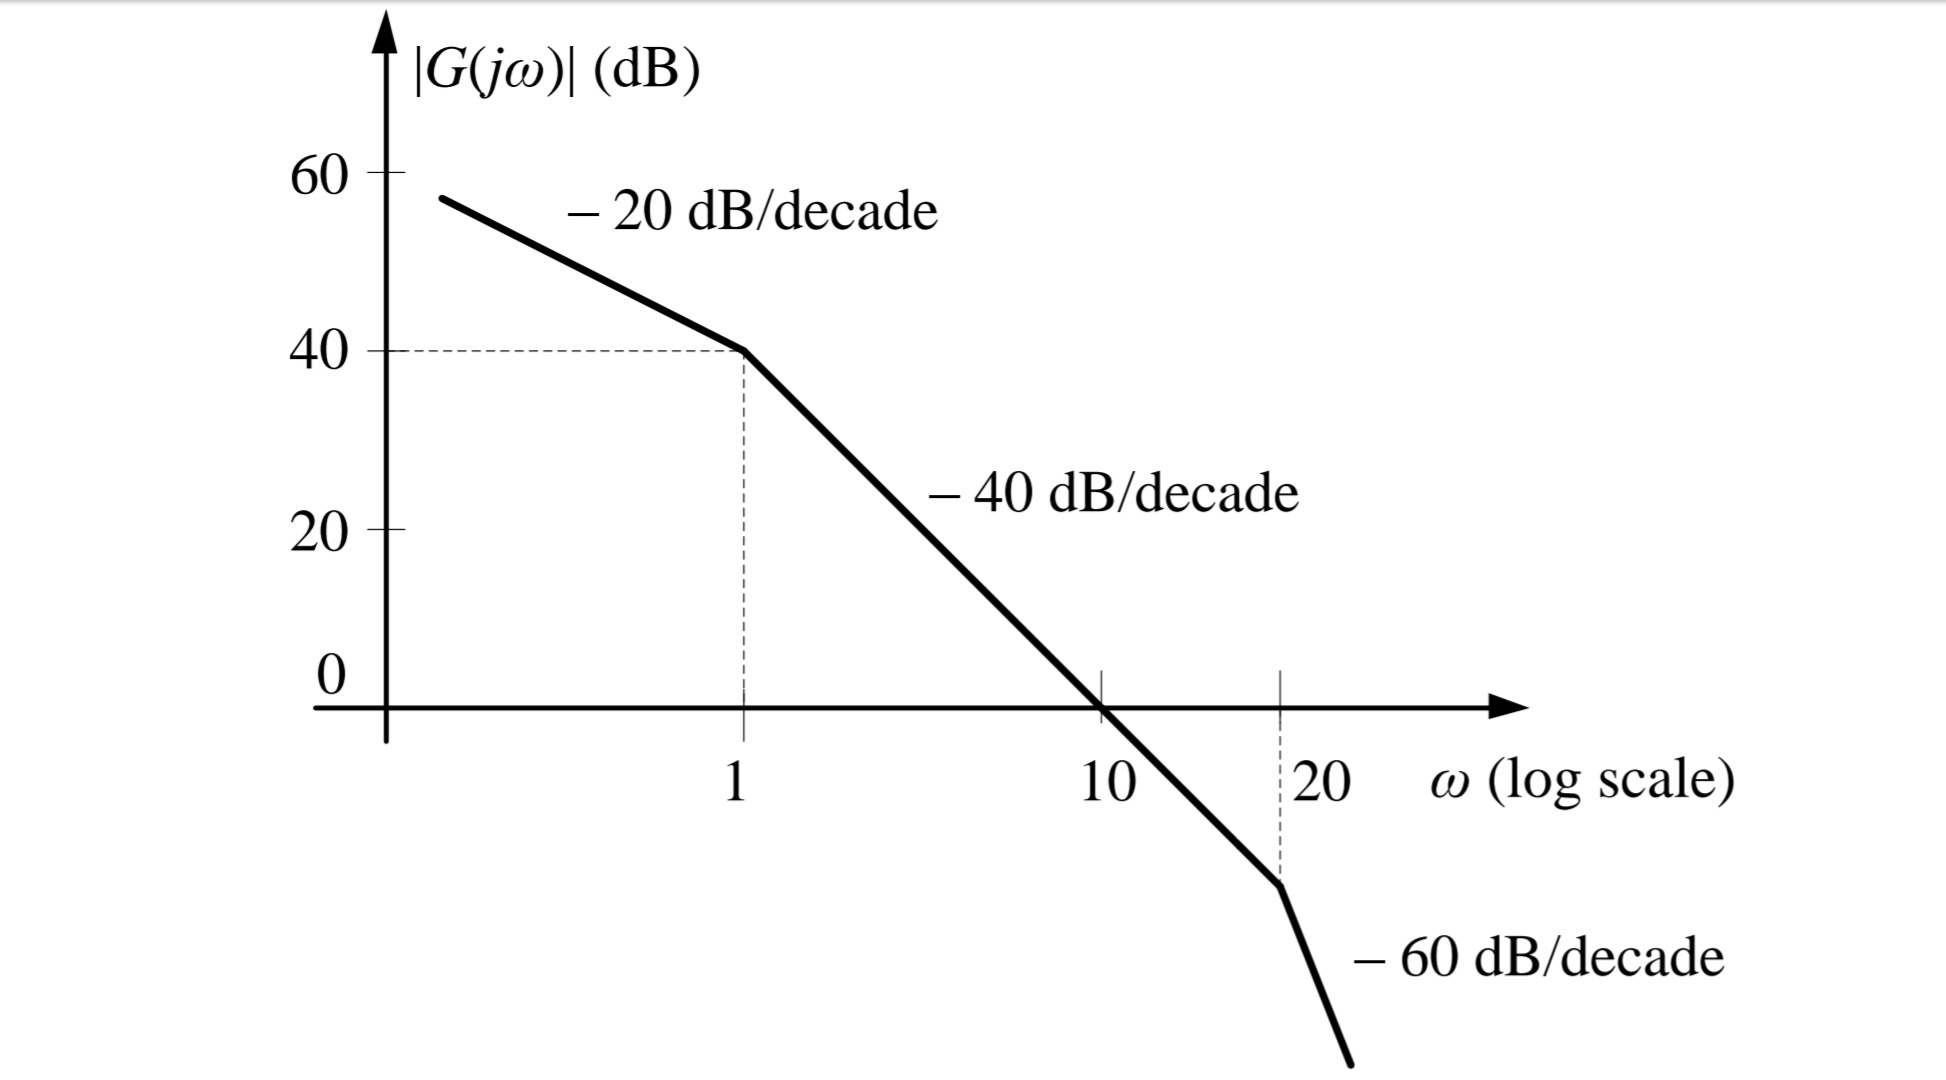
\includegraphics[scale = .15]{pppp}
\end{frame}


\begin{frame}
    


Consider the following two statements.\\
\quad Statement 1: Transfer function G(s) has 3 poles and one zero \\
\quad Statement 2: At very high frequency $(\omega \to \infty)$, the phase \\  \quad \quad \quad \quad \quad \quad angle $ \angle G(j\omega)=-3\pi/2$ \\ 
Which of the following is correct ? \\
(A) Statement 1 is true and Statement 2 is false.\\
(B) Statement 1 is false and Statement 2 is true.\\
(C) Both the statements are true.\\
(D) Both the statements are false.
\end{frame}

%------------------------------------------------

\begin{frame}
\frametitle{Solution}

Since, each pole corresponds to -20 dB/decade  
and each zero corresponds to +20 dB/decade.\\
Therefore, from the given Bode plot we can get the Transfer equation,\\
\[ G(s) = \frac{k}{s(1+s)(20+s)} \]
\\
Now, from the Transfer equation we can conclude that,
there are three poles (0, -1 and -20 ) and no zeros.\\
\quad \quad \quad $\therefore$ Statement 1 is false \quad \quad \quad ..........(1)




\end{frame}

%------------------------------------------------


\begin{frame}{Calculating phase}
Since we know that,\\
phase $ \phi $ is the sum of all the phases corresponding to each pole and zero.\\
phase corresponding to pole is = \[ - tan^{-1}( \frac{imaginary}{real}) \]
phase corresponding to zero is = \[tan^{-1}( \frac{imaginary}{real})\]

\end{frame}
%------------------------------------------------



now take,\[  s = j\omega  \]\\

 \[ \Rightarrow  G(j\omega) =  \frac{k}{j\omega(1+j\omega)(20+j\omega)}\]
 \\
Therefore, \\
 \[  \phi =  -tan^{-1}( {\frac{\omega}{0}}) - tan^{-1}(\omega) - tan^{-1}( \frac{\omega}{20})\]

  \[ \phi =  - 90^\circ - tan^{-1}(\omega) - tan^{-1}( \frac{\omega}{20})\]
  \\
  \[\because \omega \to \infty\] 


 
 \begin{frame}
  \[ \phi =   - 90^\circ - 90^\circ - 90^\circ\]
 \[\phi = -270^\circ\ \]
 \[\phi = -3\pi/2 \] 
\quad \quad \quad $\therefore$ Statement 2 is true \quad \quad \quad \quad ........(2)\\
 thus, from (1) and (2) option (B) is correct.
\end{frame}
%------------------------------------------------


\begin{frame}
\Huge{\centerline{Thank You}}
\end{frame}
\end{document}